\documentclass[12pt,a4paper,notitlepage]{article}

\usepackage[utf8]{inputenc}

\usepackage[francais]{babel}\usepackage[T1]{fontenc}
\usepackage[cyr]{aeguill}
\usepackage{lmodern}
\usepackage{color}
\usepackage{boites}
\usepackage{caption}
\usepackage{fancybox}
\usepackage{listings}
\usepackage{multicol}
\usepackage[table]{xcolor}

\usepackage[T1]{fontenc}
\usepackage[scaled]{helvet}
\renewcommand*\familydefault{\sfdefault}

%\lstset{language=bash, basicstyle=\footnotesize, frame=shadowbox, rulesepcolor=\color{gris}, captionpos=b}

  \lstset{
         basicstyle=\footnotesize\ttfamily, % Standardschrift
         %numbers=left,               % Ort der Zeilennummern
         numberstyle=\tiny,          % Stil der Zeilennummern
         %stepnumber=2,               % Abstand zwischen den Zeilennummern
         numbersep=5pt,              % Abstand der Nummern zum Text
         tabsize=2,                  % Groesse von Tabs
         extendedchars=true,         %
         breaklines=true,            % Zeilen werden Umgebrochen
         keywordstyle=\color{red},
                frame=b,         
         keywordstyle=[1]{\itshape}{//},    % Stil der Keywords
         stringstyle=\color{white}\ttfamily, % Farbe der String
         showspaces=false,           % Leerzeichen anzeigen ?
         showtabs=false,             % Tabs anzeigen ?
         xleftmargin=5pt,
         framexleftmargin=1pt,
         framexrightmargin=5pt,
         %numbers=left,
         frame=toplines,
         framextopmargin=3pt,
       %  framexleftmargin=8pt,
         numberblanklines=false,
         %morecomment=[s][marron]{/*}{*/},
         %moredelim=*[s][\color{blue}]{/*}{*/}
         %morecomment=[s][marron]{/*-}{*/}},         
         framexbottommargin=5pt,
         captionpos=b,
         %backgroundcolor=\color{lightgray},
         showstringspaces=false      % Leerzeichen in Strings anzeigen ? 
 }

\DeclareCaptionFont{white}{\color{white}}
\DeclareCaptionFormat{listing}{\colorbox[cmyk]{0.43, 0.35, 0.35,0.01}{\parbox{\textwidth}{\hspace{10pt}#1#2#3}}}
\captionsetup[lstlisting]{format=listing,labelfont=white,textfont=white, singlelinecheck=false, margin=0pt, font={bf,footnotesize}}

\definecolor{gris}{gray}{0.75}
\definecolor{bleup}{HTML}{258EE9}


%\renewcommand*\familydefault{\ttdefault} %% Only if the base font of the document is to be typewriter style
%\renewcommand{\rmdefault}{ptm}


\usepackage[
   pdfauthor={Ludovic Terrier & Arnaud Goulut},
   pdftitle={RE12 - TP6},
   ]{hyperref}
   
   
\usepackage[pdftex]{graphicx}

%\usepackage{titlesec}
%\titleformat{\section}[frame] {\normalfont} {\filright
%\footnotesize
%\enspace\textbf{\thesection}\enspace} {8pt} {\Large\bfseries\filcenter}

%% Je contrôle la taille de ma zone imprimée...
\usepackage{anysize}
%% ...en définissants les marges {gauche}{droite}{haute}{basse}
\marginsize{25mm}{15mm}{10mm}{15mm}

\begin{document}

\title{Gestion de réseau par SNMP}
\author{Ludovic Terrier et Arnaud Goulut}
\date{Juin 2010}
\maketitle


%\tableofcontents

\thispagestyle{empty}


 
%%%%%%%%%%%%%%%%%%%%%%%%%%%%%%%%%%% 1ère partie
\section{Configuration et prise en main de l'agent SNMP}

\subsection{Installation d'un agent snmp}
L'agent \texttt{net-snmp} était déjà installé lorsque nous avons pris possession de la salle de TP, il nous a donc simplement fallut éditer le fichier de configuration \textit{snmpd.conf} pour le faire fonctionner comme nous le désirions :
\begin{lstlisting}[title=snmpd.conf]
rocommunity publicB3
rwcommunity privateB3
\end{lstlisting}

Nous avons fait au plus simple, ainsi la communauté \textbf{publicB3} est autorisée a consulter les informations contenues dans la \textit{MIB}\footnote{Management Information Base}, alors que \textbf{privateB3} peut lire, mais aussi écrire dans cette même base.


\paragraph{}Cependant il restait à installer les utilitaires en ligne de commande afin d'effectuer les tests qui suivront, via la commande :\\

\noindent \texttt{yum install net-snmp-libs net-snmp-utils}

\paragraph{}Le paquet net-snmp-utils regroupe l'ensemble des outils nécessaire pour tester le bon fonctionnement de la supervision de son réseau tel que : snmpwalk, snmpget\ldots 
\subsection{Ligne de commande}
Les différents outils disponibles dans le paquet précédemment installé permettent de consulter les MIB. On utilise généralement, le nom de la commande, suivi de \texttt{-v 2c} pour la version, \texttt{-c communauté} pour la communauté avec laquelle on veut accéder à la MIB, l'adresse de la machine qui possède la MIB et enfin, l'OID sur lequel on veut appliquer la commande. Voici la liste de ces outils accompagnés d'exemples :\\




\subsubsection{\texttt{snmpget}}
Cette commande permet de récupérer uniquement la valeur d'un OID (d'une instance) précis. Ainsi, si nous voulons récupérer la personne à contacter pour un équipement donné (ici, notre machine) on utilisera :\\

\noindent \texttt{snmpget -v 2c -c publicB3 127.0.0.1 1.3.6.1.2.1.1.4.0}


\subsubsection{\texttt{snmpgetnext}}
Cet outil permet de récupérer la valeur de l'instance suivant directement celle que l'on a donnée en paramètre. Ainsi pour récupérer la valeur de l'uptime en donnant l'OID situé avant dans l'arbre :\\

\noindent \texttt{snmpgetnext -v 2c -c publicB3 127.0.0.1 1.3.6.1.2.1.1.2}

\subsubsection{\texttt{snmpwalk}}
Cet outil permet de récupérer des informations d'un sous-arbre à partir d'un point donné dans l'arbre des OIDs. Pour cela il utilise les requêtes \texttt{get-next-request} et \texttt{get-response} afin de parcourir l'ensemble des items du sous arbre donné.

\subsubsection{\texttt{snmptable}}
Cet outil permet de récupérer un ensemble d'informations en une seule commande, en le mettant sous forme d'un tableau. On lui indique un OID et la commande récupère la valeur des OIDs situés juste dessous :\\

\begin{lstlisting}[title=Résultat snmptable pour les connexions TCP]
root@pc05-d202 snmp]# snmptable -v 2c -c publicB3 127.0.0.1 1.3.6.1.2.1.6.13
SNMP table: TCP-MIB::tcpConnTable

tcpConnState tcpConnLocalAddress tcpConnLocalPort tcpConnRemAddress tcpConn
    listen             0.0.0.0              111           0.0.0.0        0
    listen             0.0.0.0            10000           0.0.0.0        0
    listen             0.0.0.0            48781           0.0.0.0        0
    listen           127.0.0.1               25           0.0.0.0        0
    listen           127.0.0.1              199           0.0.0.0        0
  established      192.168.3.1            39628     188.165.75.23       22
\end{lstlisting}
\paragraph{}Les informations qui pourraient êtres intéressant de récupérer dans une MIB sont le contact, le nom de la machine (host) et la quantité d'octets entrant et sortant pour une interface donnée. Dans une MIB on récupère généralement des \textit{métriques}, c'est ensuite à l'administrateur de les transformer en informations exploitables, on parle alors de \textit{indicateurs}. C'est par exemple le cas lorsque l'on obtient la quantité d'octets sortie d'une interface et qu'on transforme cette valeur en débit.

\paragraph{}Voici un extrait graphique de la RFC 1214 décrivant le contenu de la MIB :

\begin{figure}[!h]
\begin{center}
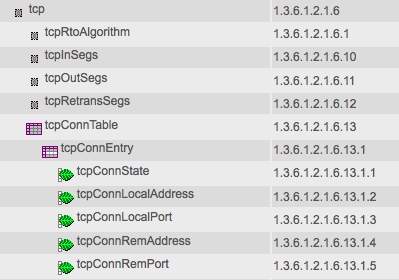
\includegraphics[height=5cm]{rfc1214.png}
\caption{Sous-arbre de la MIB au niveau des connexions TCP.}
\label{fig:rfc1214}
\end{center}
\end{figure}

On voit qu'elle est composée, de tables, d'éléments qui ne sont pas forcément des instances, mais aussi des instances concernant un OID.

\paragraph{}Nous avons ensuite récupéré une table via \textit{SNMP v1}, puis par \textit{SNMP v2c}. Nous avons pu observer via Wireshark qu'avec la v1 de SNMP, \texttt{snmptable} procède en utilisant \texttt{snmpgetnext} pour parcourir l'ensemble de la table, alors qu'avec la v2c, \texttt{snmptable} procède avec \texttt{getbulkrequest} pour récupérer plus rapidement les données.

\subsection{MibBrowser}
Ce logiciel permet de visualiser graphiquement l'ensemble de l'arbre et des valeurs associées à chaque OIDs.

\paragraph{}Dans la mesure ou le logiciel ne fonctionnait pas très bien, nous ne l'avons pas utilisé pour cette partie du TP. En effet en utilisant la fonction \texttt{snmpget}, il parcourait l'ensemble de l'arborescence au lieu de se cantonner à la requête qui lui était passée. Ainsi nous ne sommes pas en mesure de vous proposer la réponse à la présente question.

\section{Surveillance des équipements réseau et alarmes}
\subsection{Configuration équipements}
Nous avons donc tu configurer les agents SNMP de nos équipements afin d'utiliser SNMP.\\
\begin{lstlisting}[title=Commandes Cisco pour configurer l'agent SNMP du routeur]
Router3(config)# snmp-server contact Arnaud Goulut
Router3(config)# snmp-server location Salle de TP, D202
Router3(config)# snmp-server community publicB3
\end{lstlisting}

\paragraph{} Pour vérifier le bon fonctionnement, on utilise snmpwalk pour récupérer les informations de la partie \texttt{system} de la MIB :

\begin{lstlisting}[title=Vérification du fonctionnement SNMP sur le routeur]
root@pc05-d202# snmpwalk -v 2c -c publicB3 192.168.3.126 1.3.6.1.2.1.1
SNMPv2-MIB::sysDescr.0 = STRING: Cisco IOS Software, 2800 Software
Technical Support: http://www.cisco.com/techsupport
SNMPv2-MIB::sysObjectID.0 = OID: SNMPv2-SMI::enterprises.9.1.576
DISMAN-EVENT-MIB::sysUpTimeInstance = Timeticks: (682232) 1:53:42.32
SNMPv2-MIB::sysContact.0 = STRING: Arnaud
SNMPv2-MIB::sysName.0 = STRING: Routeur3
SNMPv2-MIB::sysLocation.0 = STRING: salle de tp
\end{lstlisting}

\subsection{Perte de connectivité}
Sur nos équipement, on doit donc activer l'émission de trap pour prévenir directement notre serveur de supervision.

\begin{lstlisting}[title=Activation des traps pour l'état des liens]
Router3(config)# snmp-server host 192.168.3.1 version 2c publicB3
Router3(config)# snmp-server enable traps snmp linkdown linkup coldstart warmstart
\end{lstlisting}

\paragraph{} La première ligne permet de définir l'adresse du serveur qui recevra les notifications, ainsi que la communauté qui doit être utilisée. La seconde permet de préciser sur quels événements les traps seront envoyées, ici uniquement en rapport avec les états des liens.

\subsection{Le démon snmptrapd}
Dans cet partie, nous allons configurer notre serveur pour qu'il accepte les traps qui seront émises par nos équipements réseaux. Pour cela, il faut configurer le démon snmptrapd via le fichier \texttt{/etc/snmp/snmptrapd.conf} :

\begin{lstlisting}[title=Activation des traps pour l'état des liens]
doNotRetainNotificationLogs yes
disableAuthorization yes
traphandle default /tmp/exec-trap.sh
\end{lstlisting}

\paragraph{} Trois paramètres sont donc utilisés : 
\begin{itemize}
\item doNotRetainNotificationLogs : empêche snmptrapd de garder des logs,
\item disableAuthorization : on récupérere toutes les traps, quelque soit la communauté,
\item traphandle : l'action faite lorsqu'une trap est reçue (ici un script).
\end{itemize}


\section{Prise en main d'une console de supervision}
\subsection{Installation de ZenOSS}
L'installation de ZenOSS se fait simplement, on récupère le fichier d'installation sur le site Zenoss et on le lance. Après avoir répondu à quelques questions, le tout est en place et fonctionnel. Il suffit alors d'intégrer nos équipements en indiquant notamment leur communauté d'accès et leur adresse IP, il faut aussi indiquer la \textit{classe} de l'appareil, en effet Zenoss permet d'interpréter les traps issus de MIBs propriétaires, pour se faire il faut lui signifier le type de matériel à traiter. Ainsi, Zenoss propose les classes : Cisco, serveurs (classés par systèmes d'exploitation), routeurs (par marques), etc.

\paragraph{}Cette plate-forme de supervision, permet de visualiser les traps émanant d'un réseau administré. Il suffit d'y intégrer nos équipements pour que ce logiciel reçoive les traps, les interprète selon la classe qu'on lui a indiquée et enfin les affiche dans une console.

\subsection{Parcours des fonctionnalités}


%\paragraph{}Voici le schéma décrivant l'infrastructure du réseau que nous désirons obtenir :
%\clearpage%
%\begin{figure}[!h]
%\begin{center}
%\includegraphics[height=5cm]{}
%\caption{Structure du réseau}
%\label{fig:da}
%\end{center}
%\end{figure}
\end{document}